\begin{frame}
    \frametitle{\problemtitle}

    \begin{columns}
        \begin{column}[T]{.70\textwidth}
            \begin{itemize}
                \item $n \leq 10^5$ people visit a restaurant and need to pay.
                \item Each person has their own share $b_i$ and an amount of cash $a_i$.
                \item One person will pay the entire bill and receive the cash from all others.
                \item Choose that person so they do not have to pay more than their own share $b_i$.
                \item There may be no such person.
            \end{itemize}
            %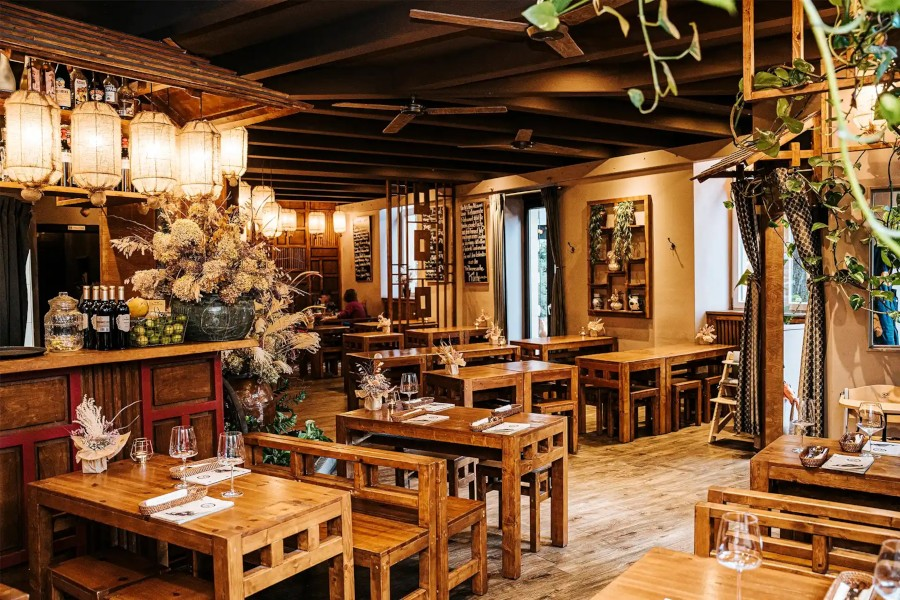
\includegraphics[width=0.25\textwidth]{vietaroma-small.jpeg}


            %\small
            %Illustration of Sample Input 1.
        \end{column}

        \illustration{0.25}{restaurant.jpg}{
            KIT teams having a celebration dinner after NWERC.\\
            Photo by Christopher Weyand
        }

    \end{columns}
\end{frame}
